%\documentclass[a4paper]{report}
%\usepackage{a4wide}
\documentclass{scrreprt}

% Allow direct typing of ä, ö, ü, for example in "Büchi"
\usepackage[utf8]{inputenc}
\usepackage{amssymb}
\usepackage{tikz}
\usetikzlibrary{automata,positioning,arrows,shapes,matrix}

\newcommand{\om}{{$\omega$}}

\tikzset{
  font=\scriptsize\sffamily
}

\begin{document}
% Title page
\title{Investigation on the Performance of a Subset-Tuple Büchi Complementation Construction}
\author{Daniel Weibel}
\date{\today}
\maketitle

% Abstract
% \begin{abstract}
% Hello world
% \end{abstract}

% Table of contents
\tableofcontents

\chapter{Introduction}

% Context of study
A Büchi complementation construction takes as input a Büchi automaton $A$ and produces as output another Büchi automaton $B$ which accepts the complement language of the input automaton $A$. Complement language denotes the ``contrary'' language, that is, $B$ must \emph{accept} (over a given alphabet) every word that $A$ \emph{does not} accept, and must in turn \emph{not accept} every word that $A$ \emph{accepts}.

Büchi automata are finite automata (that is, having a finite number of states) which operate on infinite words (that is, words that ``never end''). Operating on infinite words, they belong thus to the category \om-automata. An important application of Büchi automata is in model checking which is a formal system verification technique. There, they are used to represent both, the description of the system to be checked for the presence of a correctness property, and (the negation of) this correctness property itself.

In one approach to model checking, the correctness property is directly specified as a Büchi automaton
One approach to model checking requires that the Büchi automaton representing the correctness property is complemented. It is here that the problem of Büchi complementation has one of its practical applications. 

% Stating the problem, reason the research is worth tackling
The complementation of non-deterministic Büchi automata is hard. It has been proven to have an exponential lower bound in the number of generated states [cite]. That is, the number of states of the output automaton is, in the worst case, an exponential function of the number of states of the input automaton. However, since the introduction of Büchi automata in the 1960's, significant process in reducing the complexity (in other words, the degree of exponentiality) of the Büchi complementation problem has been made. Some numbers [list complexities of the different constructions].

% Aim and scope

% Significance: advance knowledge, contribute to solutin of practical problem, novel use of a procedure or technique?

% Overview

\chapter{Background}
\section{Büchi Automata}
\subsubsection{Definition}
Informally speaking, a Büchi automaton is a finite state automaton running on input words of infinite length. That is, once started reading a word, a Büchi automaton never stops. A word is accepted by a Büchi automaton, if there exists a run (sequence of states) for it that includes infinite repetitions of at least one accepting state. In other words, if during reading a word a Büchi automaton goes through one or more accepting states infinitely often, the word is accepted, and otherwise it is rejected.

More formally, a Büchi automaton $A$ consists of a 5-tuple $A = (\Sigma, Q, q_0, \delta, F)$, the components of which are the following.
\begin{itemize}
\item $\Sigma$: a finite alphabet
\item $Q$: a finite set of states
\item $q_0$: an initial state, $q_0 \in Q$
\item $\delta$: a transition function $q: Q \times \Sigma \rightarrow 2^Q$ %(mapping combinations of a state and a symbol to zero, one, or more other states)
\item $F$: a set of accepting states, $F \in 2^Q$
\end{itemize}

This is so far the same definition as for normal finite state automata. What distinguishes a Büchi automaton from a normal finite state automata is its acceptance condition. To define the Büchi acceptance condition, we first have to define the following notions.

\begin{itemize}
\item $\Sigma^\omega$ isthe set of all possible words of infinite length over an alphabet $\Sigma$
\item A \emph{run} of Büchi automaton $A$ on a word $x \in \Sigma^\omega$ is a sequence of states $q_0q_1q_3\dots$ such that $q_0$ is $A$'s initial state and $\forall i \geq 0: q_{i+1} \in \delta(q_i, x_i)$
\item $\textrm{inf}(\rho) \in 2^Q$ is the subset of states of $Q$ that occur infinitely often in a run $\rho$
\item An \emph{accepting run} is a run $\rho$ for which $\textrm{inf}(\rho) \cap F \neq \varnothing$  
\end{itemize}

A word $x \in \Sigma^\omega$ is then accepted by a Büchi automaton $A$ if and only if there exists an accepting run of $A$ on $x$.

\subsubsection{Deterministic and Non-Deterministic Büchi Automata}
As for normal finite state automata, there are deterministic and non-deterministic versions of Büchi automata. The difference lies in the transition function. For the non-deterministic case it is $\delta: \Sigma \times Q \rightarrow 2^Q$, but for the deterministic case it is strictly $\delta: \Sigma \times Q \rightarrow Q$. That means, whereas in a non-deterministic Büchi automaton a state $q$ may have zero, one, or more successors on a given symbol $a$ (denoted by $\delta(q,a) \geq 0$), in a deterministic Büchi automaton this number is always exactly one ($\delta(q,a) = 1$).

The definition of a Büchi automaton given above is thus in fact the definition of a non-deterministic Büchi automaton. This coincides with a convention that we adopt in this thesis. If not explicitly stated, when we say ``Büchi automaton'' we actually mean a non-deterministi Büchi automaton. This is first, because deterministic Büchi automata are a special case of non-deterministic Büchi automata, and second, the problem of complementation that this thesis is about is only significant for the non-deterministic case.

A Büchi automaton is complete if every state has at least one outgoing transition for every symbol of the alphabet. Formally, this means that $|\delta(q,a)| \geq 1, \forall q \in Q, \forall a \in \Sigma$. Note that deterministic Büchi automata are always complete, and thus only non-deterministic Büchi automata can be incomplete

\subsubsection{Equivalences}
An important property of Büchi automata is that deterministic Büchi automata are less expressive than non-deterministic Büchi automata. That means that there exist non-deterministic Büchi automata for which no deterministic Büchi automata accepting the same language exists.

Non-deterministic Büchi automata in turn are equivalent to the \om-regular languages. That means that every language that is recognised by any Büchi automaton is an \om-regular language, and for every \om-regular language there exists a non-deterministic Büchi automaton recognising it.

Furthermore, non-deterministic Büchi automata are equivalent to other classes of \om-automata such as Muller, Rabin, Streett, and Parity automata. Within these classes, determinstic and non-deterministic automata are equivalent. This means that every Büchi automaton can be translated to an equivalent deterministic or non-deterministic Muller, Rabin, Streett, or Parity automaton, and any of these latter automata can be translated to a non-deterministic Büchi automaton. Figure~\ref{equivalences} summarises these expressive relations of Büchi automata.

\begin{figure}[htb]
\begin{center}
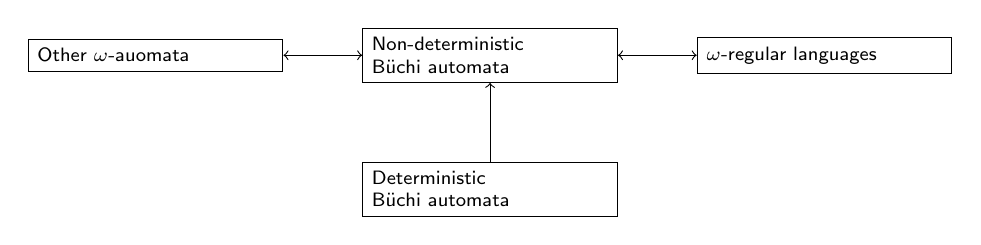
\begin{tikzpicture}[item/.style={rectangle,draw,text width=3cm}]
\node[item] (left) {Other \om-auomata};
\node[item] (middle) [right=of left] {Non-deterministic\\Büchi automata};
\node[item] (right)  [right=of middle] {\om-regular languages};
\node[item] (bottom) [below=of middle] {Deterministic\\Büchi automata};
\path[<->] (left) edge (middle)
           (middle) edge (right);
\path[->] (bottom) edge (middle);
\end{tikzpicture}
\caption{Expressive relations of Büchi automata.}
\label{equivalences}
\end{center}
\end{figure}

\subsection{Complementation of Büchi Automata}
It has been proved by Büchi himself that Büchi automata are closed under complementation [cite Büchi]. That means that for every Büchi automaton, there exists another Büchi automaton accepting the complement language of the initial automaton.

Let us denote by $L(A)$ the language recognised by Büchi automaton $A$. Then the complement language $\overline{L(A)}$ of $L(A)$ is $\overline{L(A)} = \Sigma^\omega \setminus L(A)$.

\hbox to \hsize{\hfill{
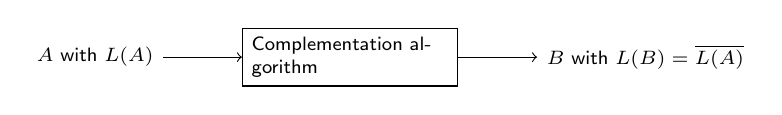
\begin{tikzpicture}[item/.style={rectangle,draw,text width=2.5cm}]
\node[] (left) {$A$ with $L(A)$};
\node[item] (middle) [right=of left] {Complementation algorithm};
\node[] (right)  [right=of middle] {$B$ with $L(B) = \overline{L(A)}$}; 
\path[->] (left) edge (middle)
          (middle) edge (right);
\end{tikzpicture}}\hfill}

The problem of Büchi complementation can thus be summarised as follows. Given a Büchi automaton $A$, find a Büchi automaton $B$, such that $L(B) = \overline{L(A}$. For solving this problem we need an algorithm that takes $A$ as input and returns $B$ as output. 

As a starting point, let us look at the complementation problem for normal finite state automata on finite words. Normal finite state automata recognise the regular languages and are also closed under complementation. For deterministic finite state automata, a possible complementation algorithm consists in simply inverting the accepting and non-accepting states of the automaton. Inuitively, every word that leaves the input automaton in an accepting state will leave the output automoaton in a non-accepting state, and vice versa. For the case of non-deterministic automata, one can take adavantage of the fact that every non-deterministic automata can be converted to an equivalent deterministic automaton. A standard algorithm for this conversion is the subset-construction, which is described in detail in [cite Hopcroft, Sec. 2.3.5]. The subset-construction basically takes all the subsets of states of the input automaton as states of the output automaton. A possible complementation algorithm for non-deterministic finite state automata consists thus in determinisation by the subset-construction and complementation by switching accepting and non-accepting states.

Again, the cases of deterministic and non-deterministic automata are treated separately. For DBW, the method of switching accepting and non-accepting states does not work. Imagine for example that $\rho$ is the run of the word $x \in \Sigma^\omega$ of automaton $A$ (a DBW has exactly one run for every word of $\Sigma^\omega$). If $\textrm{inf}(\rho)$ contains both an accepting and a non-accepting state, then the switching of accepting and non-accepting states has no effect on the acceptance of $x$, as it is accepted in both cases. A working procedure for complementing DBW has been described by Kurshan [cite Kurshan, 1987]. Kurshan's construction is relatively easy and can be described in one sentence: make all states of the input automaton $A$ non-accepting, add another copy of $A$, remove all its accepting states and make the non-accepting states accepting, and finally add transitions from the states of the first copy of $A$ to the corresponding destination states in the second copy of $A$. The resulting automaton is an NBW $B$ that accepts the complement language of the input DBW $A$.

In the case of finite-word automata, the complementation procedure for DFA provided a solution for the complementationn of NFA, because there is a translation from every NFA to an equivalent DFA. For Büchi automata this is however not the case. As mentioned above, there are NBW for which no equivalent DBW exists. We say that NBW can in general not be determinised.

\section{Review of Proposed Büchi Complementation Algorithms}
\subsection{Ramsey-Based Approaches}
\subsection{Determinisation-Based Approaches}
\subsection{Rank-Based Approaches}
\subsection{Slice-Based Approaches}

\section{The Fribourg Construction}

\section{Empirical Performance Investigation}




\chapter{The Wider Context: System Verification}
\section{Section} % Two indices, e.g. 2.1
\subsection{Subsection} % Three indices, e.g. 2.1.1
\subsubsection{Subsubsection} % No indices, not in table of contents

\chapter{The B\"uchi Complementation Problem}

\chapter{The Fribourg Construction}

\chapter{Discussion}

\chapter{Conclusions}

\end{document}